\documentclass[11pt]{standalone}
\usepackage[usenames]{color} %used for font color
\usepackage{amssymb} %maths
\usepackage{amsmath} %maths
\usepackage[no-math]{fontspec}
\usepackage{unicode-math}
\usepackage{libertinus}

\usepackage{pgf,xcolor}
\definecolor{itwm_blue}{HTML}{005A94}
\definecolor{itwm_red}{HTML}{C00000}
\usepackage{tikz}
\usepackage{pgfplots}
\pgfplotsset{compat=newest}

\pgfmathsetmacro{\ymin}{-3}
\pgfmathsetmacro{\ymax}{3}

\begin{document}
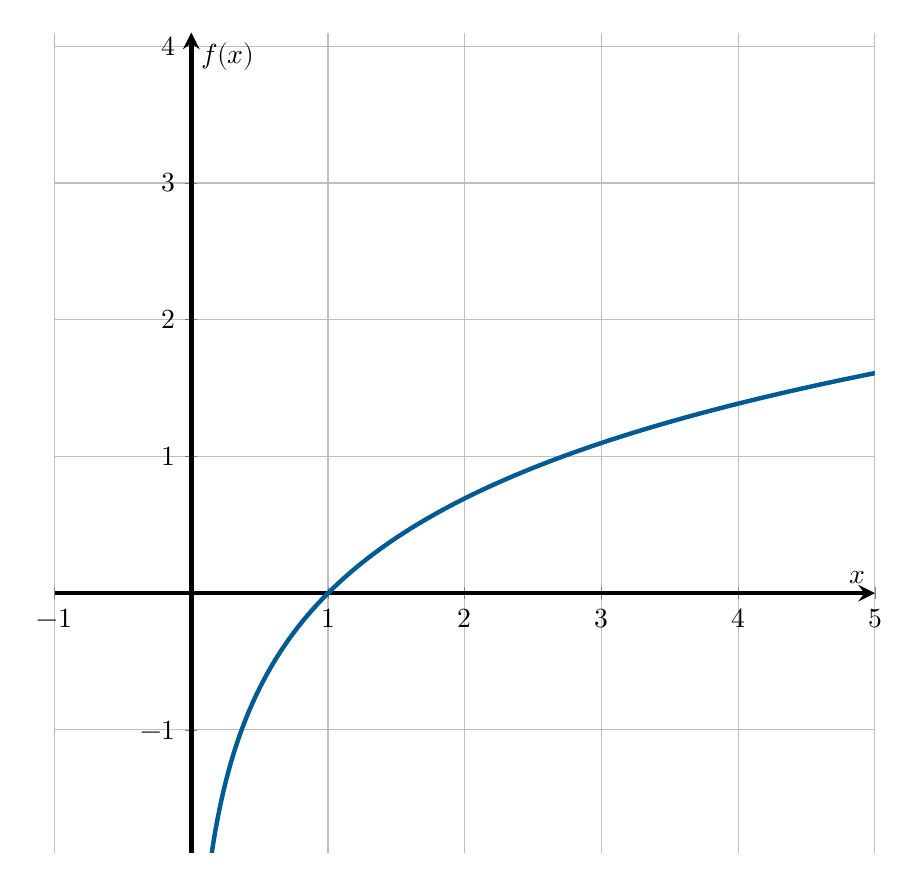
\begin{tikzpicture}
\begin{axis}[
    domain=0.01:5,
    axis lines = center,
    xlabel = {$x$},
    ylabel = {$f(x)$},
    height=12cm, width=12cm, 
    xmin=-1, xmax=5,
    ymin=\ymin*1.1, ymax=\ymax*1.1,
    grid = both,
    axis equal,
    axis line style={ultra thick},
]
    
\addplot[draw=itwm_blue, samples=300, ultra thick]{ln(x)};

\end{axis}
\end{tikzpicture}
\end{document}